\chapter{Experiments} \label{chap:experiments}
\vspace{-0.05in}
The convergence guarantees presented in the previous chapter comes with requirements on the meta-parameters (\ie $\alpha$ and $m$) that may be too conservative for practical applications.
Here we provide a practical and automatic way to choose the step size $\alpha$ and the number of sub-iterations $m$ performed between snapshots.
Additionally, we exploit a variance-reduction technique for importance weighting.
Despite lacking theoretical guarantees for the variant proposed in this chapter, we will show that this method can outperform the baseline \acs{SVRPG} (Algorithm~\ref{alg:svrpg}) over deep \acs{RL} tasks coming from the literature.

\vspace{-0.05in}
\section{Full Gradient Update}
\vspace{-0.05in}
As noted in \hyperref[chap:algorithm]{Chapter 3}, the update performed at the beginning of each epoch is equivalent to a full-gradient update. In our setting, where collecting samples is particularly expensive, the additional $B$ trajectories collected using the snapshot trajectory $\pi_{\wt{\vtheta}^s}$ feels like a waste of data (the term $\sum_i g(\tau_i) - \omega(\tau_i) g(\tau_i) =0$ since $\vtheta_0 = \wt{\vtheta}$).
In practice, we just perform an approximate full gradient update using the $N$ trajectories sampled to compute $\gradApp{\wt{\vtheta}^s}{N}$, \ie
\begin{align*}
&\vtheta_{1}^{s+1} = \wt{\vtheta}^s + \alpha\gradApp{\wt{\vtheta}^s}{N} \\
&\vtheta_{t+1}^{s+1} = \vtheta_t^{s+1} + \alpha 
%        v_t^{s+1}
\blacktriangledown J(\vtheta^{s+1}_t)
\text{ for $t=1,\dots,m-1$}.
\end{align*}
In the following, we will always use this practical variant.

\vspace{-0.05in}
\section{Meta-Parameter Selection}\label{sec:stopping}
\vspace{-0.05in}
% In section \ref{sec:conv}, we introduced the practical need to properly choose $\alpha$ and $m$, which are, respectively, the step size and the number of sub-iterations to perform after a snapshot.
% At this point, the open question is how to properly select the step size $\alpha$ and the sub-iteration number $m$ in practical applications.
The step size $\alpha$ is crucial to balance variance reduction and efficiency, as well as
% The first parameter is crucial to balance the variance introduced by estimations within sub-iterations with respect to the variance introduced by estimations associated to the snapshots.
the epoch length $m$. The latter is able to control the variance introduced by the importance weights and to handle efficiency \wrt the number of updates. In the first case, low values of $m$ are associated with small variance, but increase the frequency of snapshot points (which means many \acs{FG} computations). High values of $m$ may move policy $\pi_{\vtheta_t}$ far away from the snapshot policy $\pi_{\wt{\vtheta}}$, causing large variance in the importance weights. Whereas, in the second case, the number of updates performed will directly increase \wrt $m$ itself. We will jointly set the two meta-parameters.
% the farther the distance between the snapshot policy and the current one, the higher the variance of the importance weights.

\textbf{Adaptive step size.}
A standard way to deal with noisy gradients is to use adaptive strategies to compute the step size.
 \ac{ADAM}~\citep{kingma2014adam} stabilizes the parameter update by computing learning rates for each parameter based on an incremental estimate of the gradient variance.
Due to this feature, we would like to incorporate \acs{ADAM} in the structure of the \acs{SVRPG} update.
Recall that \acs{SVRPG} performs two different updates of the parameters $\vtheta$: I) \acs{FG} update in the snapshot; II) corrected gradient update in the sub-iterations.
Given this structure, we use two separate \acs{ADAM} estimators:
\begin{align*}
\vtheta^{s+1}_1 &= \wt{\vtheta}^s + \alpha^{\textsc{FG}}_s\left(\wh{\nabla}_N J(\wt{\vtheta}^s) \right)\\
\vtheta^{s+1}_{t+1} &= \vtheta^{s+1}_t + \alpha^{\textsc{SI}}_{s+1,t}\left( 
%        v_t^{s+1}
\blacktriangledown J(\vtheta^{s+1}_t)\right)
\text{ for $t=1,\dots,m-1$},
\end{align*}
where $\alpha^{\textsc{FG}}_{s}$ is associated with the snapshot and $\alpha^{\textsc{SI}}_{s+1,t}$ with the sub-iterations.
\begin{algorithm}[h]
	\begin{algorithmic}
		\STATE \textbf{Input:} A gradient estimate $g_t$ and parameters $\beta_1$, $\beta_2$, $\epsilon$ and $\alpha$.
		\STATE $\kappa_t = \beta_1 \kappa_{t-1} + (1 - \beta_1) g_t$
		\STATE $\nu_t = \beta_2 \nu_{t-1} + (1 - \beta_2) g_t \circ g_t$ ($\circ$ is the Hadamard (component-wise) product)
		\STATE $\hat{\kappa}_t = \dfrac{\kappa_t}{1 - \beta^t_1}$
		\STATE $\hat{\nu}_t = \dfrac{\nu_t}{1 - \beta^t_2}$
		\STATE $\Delta(g_t) = \dfrac{\alpha}{\sqrt{\hat{\nu}_t} + \epsilon} \hat{\kappa}_t$
		\STATE \textbf{Return:} The increment $\Delta(g_t)$  of the parameters.
	\end{algorithmic}
	\caption{
		\label{A:adam}
		Adam}
\end{algorithm}
We report pseudo-code of the original \acs{ADAM} \citep{kingma2014adam} in Algorithm \ref{A:adam}. As mentioned, we use two distinct instances of \acs{ADAM} to manage different sources of variance: one related to the snapshots, and one to the sub-iterations. In this way the \acs{ADAM} associated to the snapshots takes into account only the history of gradient moments at the snapshots. By using Algorithm \ref{A:adam} as a subroutine $\textbf{ADAM}(g,\alpha,\beta)$, we can explicitly define our gradient updates:

\begin{align*}
\vtheta^{s+1}_1 &= \wt{\vtheta}^s + \textbf{ADAM}\left(\wh{\nabla}_N J(\wt{\vtheta}^s),\beta_1,\beta_2,\alpha\right),\\
\vtheta^{s+1}_{t+1} &= \vtheta^{s+1}_t + \textbf{ADAM}\Big( 
%        v_t^{s+1}
\blacktriangledown J(\vtheta^{s+1}_t),\beta_1,\beta_2,\frac{\alpha}{2}\Big)
\text{ for $t=1,\dots,m-1$},
\end{align*}

where separate histories are kept for estimated first moments $\kappa_{FG},\kappa_{IS}$ and estimated second moments $\nu_{FG},\nu_{IS}$.
The meta-parameters $\alpha,\beta_1,\beta_2$ are constant and set to default values or with minor manual tuning (see table \ref{table:metaparams}). Note that we double the learning rate for the snapshot \acs{ADAM} since we can rely on a larger number of trajectories ($N$ instead of $B$) to control the variance and the estimator in the snapshot does not require importance weights. With the approach above described, we managed to decouple the contribution of the variance due to the approximate \acs{FG} from the one introduced by the sub-iterations.\newline

\textbf{Adaptive epoch length.}
It is easy to imagine that a predefined schedule (\eg $m$ fixed in advance or changed with a policy-independent process) may poorly perform due to the high variability of the updates.
In particular, given a fixed number of sub-iterations $m$, the variance of the updates in the sub-iterations depends on the snapshot policy, the sampled trajectories and the learning rate.
Since the \acs{ADAM} estimate partially captures such variability,  we propose to take a new snapshot (\ie interrupt the sub-iterations) whenever the step size $\alpha^{\textsc{SI}}$ proposed by \acs{ADAM} for the sub-iterations is smaller than the one for the \acs{FG} (\ie $\alpha^{\textsc{FG}}$).
If the latter condition is verified, it amounts to say that the noise in the corrected gradient has overcome the information of the \acs{FG}. More precisely, this holds true because \acs{ADAM} wheights the learning rate \wrt the variance it is experiencing over the data it receive in input.
Formally, the stopping condition, which implies our algorithm becoming adaptive \wrt $m$, is as follows
\[
\textbf{If }        \frac{\alpha^{\textsc{FG}}}{N} > \frac{\alpha^{\textsc{SI}}}{B} \textbf{ then } \text{take snapshot,}
\]
where we have introduced $N$ and $B$ to take into account the trajectory efficiency (\ie weighted advantage).
The less the number of trajectories used to update the policy, the better.
Including the batch sizes in the stopping condition allows us to optimize the trade-off between the quality of the updates and the cost of performing them.
% This weighted approach comes from the fact that, as mentioned above, there is no advantage in having $m$ too small.
% Thus, we aim to facilitate sub-iterations rather than snapshots.

\vspace{-0.05in}
\section{Normalized Importance Sampling}\label{sec:prac}
\vspace{-0.05in}
As mentioned in Section~\ref{sec:stopping}, importance weights are an additional source of variance. A standard way to cope with this issue is self-normalization~\citep[\eg][]{precup2000eligibility,owenmcbook}.
This technique can reduce the variance of the importance weights at the cost of introducing some bias~\citep[][Chapter 9]{owenmcbook}.
Whether the trade-off is advantageous depends on the specific task.  
To introduce self-normalization in the context of our algorithm, we switch from Eq.~\eqref{E:svrpg.estimate.batch} to:
\begin{align*}
\blacktriangledown J(\vtheta_{t}) &= \wh{\nabla}_N J(\wt{\vtheta}) + \frac{1}{B} \sum_{i=0}^{B-1} \left[g(\tau_i|\vtheta_t)\right]\\ 
&\qquad{} - \frac{1}{\Omega} \sum_{i=0}^{B-1} \left[ \omega(\tau_i|\vtheta_t, \wt{\vtheta}) g(\tau_i|\wt{\vtheta})
\right].
\end{align*}
where $\Omega = \sum_{i=0}^{B-1}\omega(\tau_i|\vtheta_t, \wt{\vtheta})$.
In the next section we also show empirically that self-normalization can provide a performance improvement.

\vspace{-0.05in}
\section{Experimental Results}\label{sec:exp}
\vspace{-0.05in}
In this section, we evaluate the performance of \acs{SVRPG} and compare it with policy gradient on well known continuous \acs{RL} tasks: Cart-pole balancing and Swimmer~\citep[\eg][]{duan2016benchmarking}.
We consider G(PO)MDP since it has a smaller variance than REINFORCE \citep{zhao2011analysis}.
% This comparison is performed using G(PO)MDP as an estimator of $\score{\vtheta}{\tau}\Reward(\tau)$ in both cases. 
For our algorithm, we use a batch size $N=100$, a mini-batch size $B=10$, and the jointly adaptive step size $\alpha$ and epoch length $m$ proposed in Section \ref{sec:stopping}. Since the aim of this comparison is to show the improvement that \acs{SVRG}-flavored variance reduction brings to \acs{SG} in the policy gradient framework, we set the batch size of the baseline policy gradient algorithm to $B$, however, for completeness, we also report the results for a batch size equivalent to $N$ because it is the most used in the literature. In this sense, we measure the improvement yielded by computing snapshot gradients and using them to adjust parameter updates. Since we evaluate on-line performance over the number of sampled trajectories, the cost of computing such snapshot gradients is automatically taken into consideration. To make the comparison fair, we also use \acs{ADAM} in the baseline policy gradient algorithm, which we will denote simply as G(PO)MDP in the following.
In all the experiments we used deep Gaussian policies with adaptive standard deviation.
The swimmer experiment is run $20$ times with a random policy initialization and seed, but this initialization is shared among the algorithms under comparison. Cart-pole and half-cheetah are performed in the same way except for the number of times each experiment is run: $10$ times for the former and $5$ times for the latter. The length of the experiment, \ie the total number of trajectories, is fixed for each task. Performance is evaluated by using test-trajectories on a subset of the policies considered during the learning process. We provide average performance with 90\% bootstrap confidence intervals.  
Task implementations are from the \textit{rllab} library \citep{duan2016benchmarking}, on which our agents are also based.\footnote{rllab can be found at \url{https://github.com/rll/rllab}}
More details on meta-parameters and exhaustive task descriptions are now provided before reporting the actual results of our work:
\begin{enumerate}
	\item \emph{Cart-Pole Balancing} : an inverted pendulum mounted on a cart must be kept standing by moving the cart backward or forward (see figure \ref{fig:cartpoletask});4-dimensional state space: cart position x, pole angle $\theta$, cart velocity $\dot{x}$ and pole velocity $\dot{\theta}$; 1-dimensional action space: the horizontal force applied to the cart body. Reward function  is defined as $r(s, a) := 10 - (1 - cos(\theta)) - 10^{-5}\norm[] a^2$. The episodes terminate when $|x|>2.4$ or $|\theta|>0.2$ or the number of time steps T is greater than 100. This is a continuous variant of the Cart-Pole task of \cite{sutton1998reinforcement}.
	\item \emph{Mujoco Swimmer}: a snake-like robot immersed in a fluid must move forward (see figure \ref{fig:swimmertask}); 13-dimensional state space: 3 links velocities ($v_x$ and $v_y$ of center of masses) and 2 actuated joints angles. 2-dimensional action space: the two momentums applied on actuated joints.  The reward function is defined as $r(s, a) := v_x - 10^{-4}\norm[2]{a}^2$. The episodes terminate when the number of time steps T is greater than 500.
	\item \emph{Mujoco Half Cheetah}: a planar biped robot must move forward (see figure \ref{fig:halfcheetahtask}); 20-dimensional state space: 9 links and 6 actuated joints angles. 6-dimensional action space: the 6 momentums applied on actuated joints.  The reward function is defined as $r(s, a) := v_x - 0.05\norm[2]{a}^2$. The episodes terminate when the number of time steps T is greater than 500.
\end{enumerate}
\begin{figure*}[h]
	\begin{minipage}[t]{0.32\textwidth}
		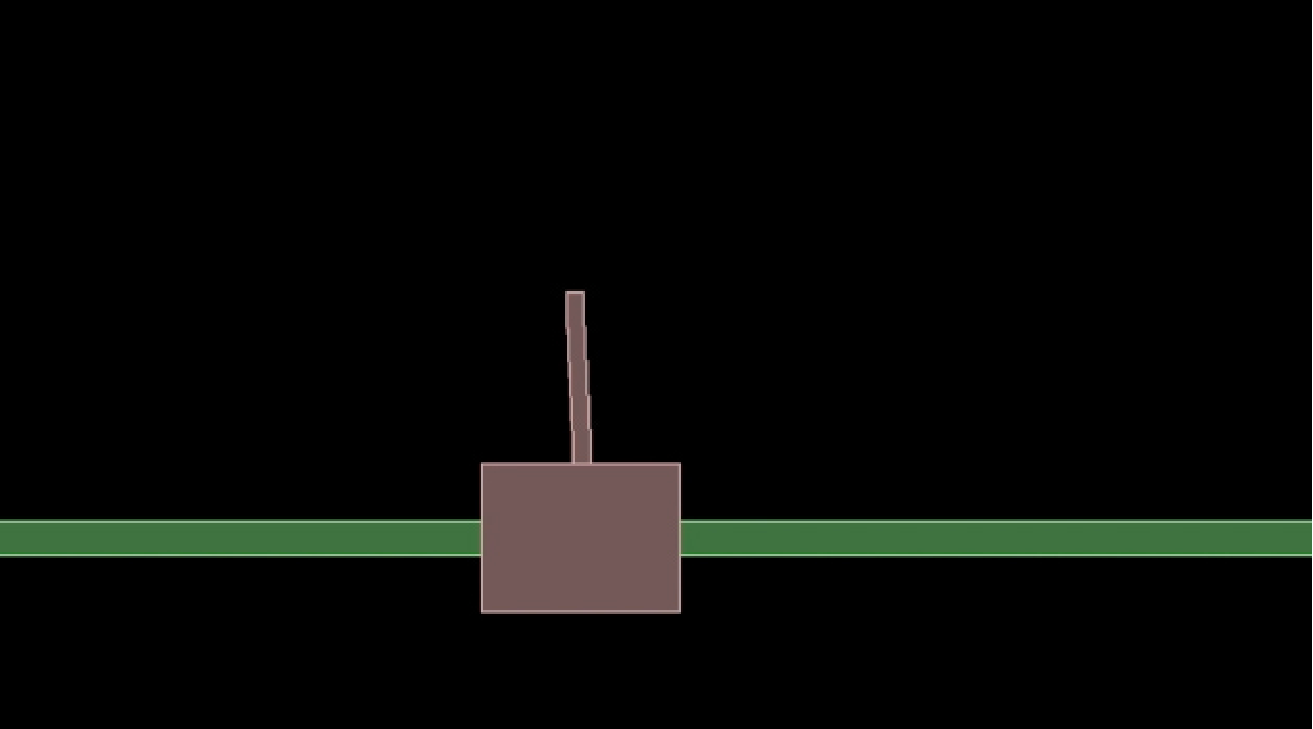
\includegraphics[width=1\textwidth]{Images/Experiments/cart.pdf}
		\vspace{-0.1in}
		\caption{Cart-Pole}
		\label{fig:cartpoletask}
	\end{minipage}
	\begin{minipage}[t]{0.32\textwidth}
		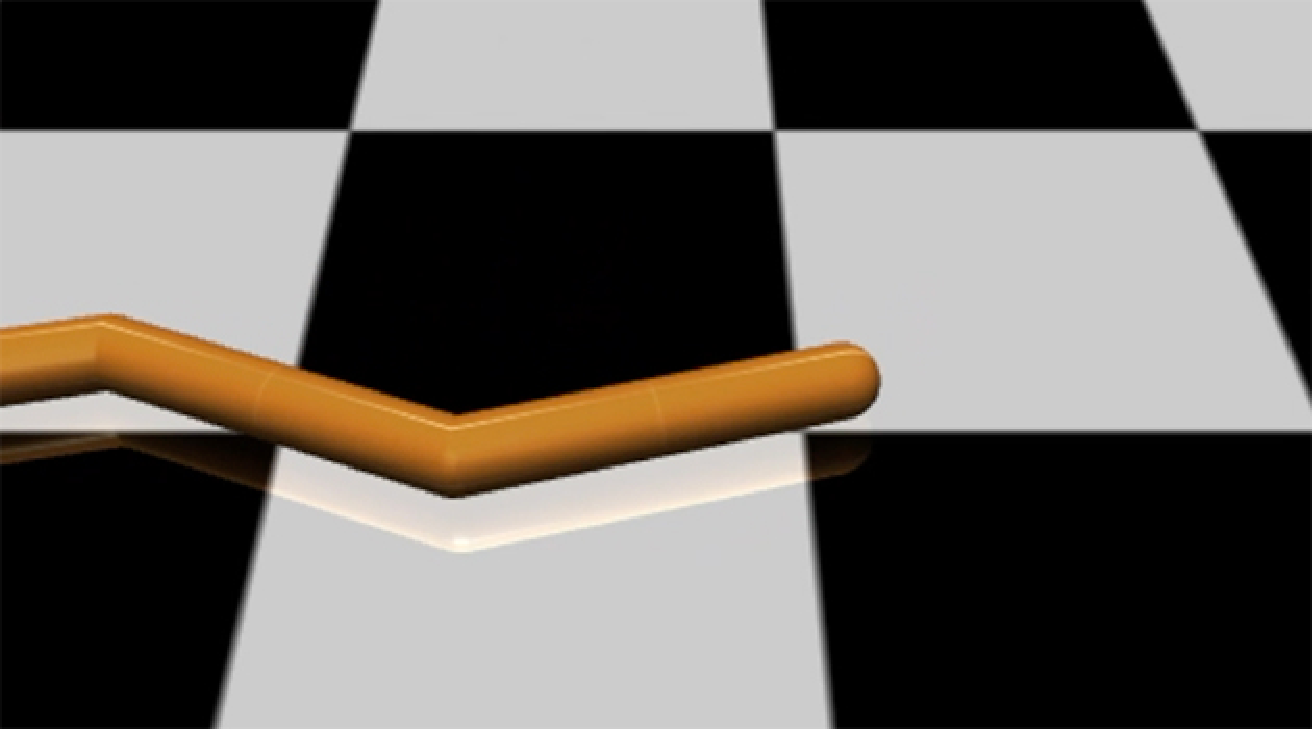
\includegraphics[width=1\textwidth]{Images/Experiments/swimmer.pdf}
		\vspace{-0.1in}
		\caption{Swimmer}
		\label{fig:swimmertask}
	\end{minipage}
	\begin{minipage}[t]{.34\textwidth}
		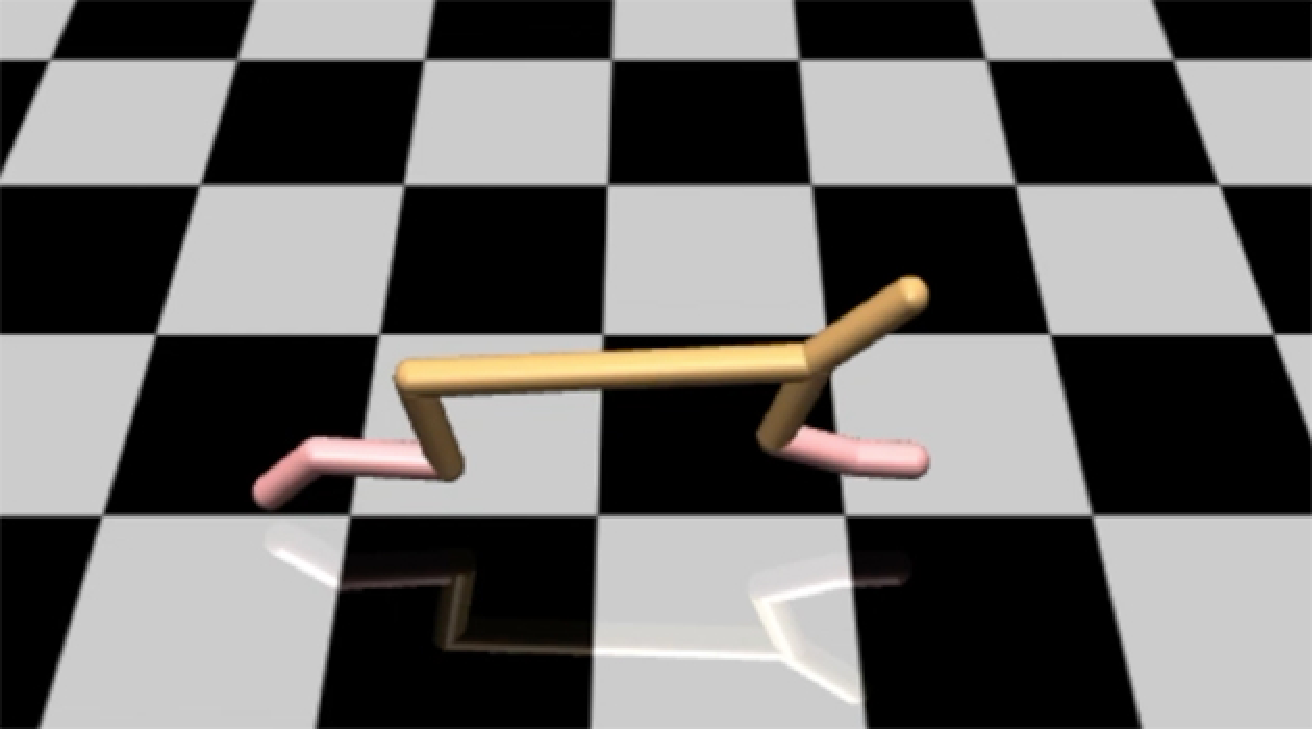
\includegraphics[height=60,width=1\textwidth]{Images/Experiments/half.pdf}
		\vspace{-0.1in}
		\caption{Half-Cheetah}
		\label{fig:halfcheetahtask}
	\end{minipage}
	\vspace{-0.15in}
\end{figure*}

All the parameters used in the experiments, including neural network architectures, are reported in the following table:

\begin{table}[H]\caption{Parameters used in the experiments. Where not specified, meta-parameters are shared among G(PO)MDP and SVRPG.}\label{table:metaparams}
	\centering
	\begin{tabular}{| l | c  c  c |}
		\hline	
		& Cart-Pole & Swimmer & Half Cheetah \\
		\hline
		NN hidden weights & 8 & 32x32 & 100x50x25 \\
		NN activation & tanh & tanh & tanh \\
		Adam $\alpha$ (SVRPG) & $5\cdotp10^{-2}$ & $10^{-3}$ & $10^{-3}$ \\
		Adam $\alpha$ (GPOMDP) & $10^{-2}$ & $10^{-3}$ & $10^{-2}$ \\
		Adam $\beta_1$ & 0.9 & 0.9 & 0.9 \\
		Adam $\beta_2$ & 0.99 & 0.99 & 0.99 \\ 
		Snapshot batch size $N$ (SVRPG) & 100 & 100 & 100 \\
		Mini-batch size $B$ (SVRPG) & 10 & 10 & 10 \\
		Batch size (GPOMDP) & 10 or 100 & 10 or 100 & 10 or 100\\
		Max number of sub-iterations & 50 & 20 & 20 \\
		Task horizon& 100 & 500 & 500 \\
		Baseline& No & No & Yes \\
		Discount factor $\gamma$& 0.99 & 0.995 & 0.99 \\
		Total number of trajectories& 10000 & 20000 & 50000 \\
		\hline  
	\end{tabular}
\end{table}
Let us be a little bit more precise about the neural network role: given an observation it will predict mean and standard deviation of the gaussian distribution from which we will need to sample our action. Refer to \cite{duan2016benchmarking} for more details about G(PO)MDP (REINFORCE in the paper) on the Half Cheetah task.


Now we can properly anddress the main results of our work. Figure \ref{fig:cartpole} compares \acs{SVRPG} versus G(PO)MDP with batch size set to $10$ on a continuous variant of the classical Cart-pole task, which is a 2D balancing task. Despite using more trajectories on average for each parameter update, our algorithm shows faster convergence, which can be ascribed to the better quality of updates due to variance reduction. The same can be said \wrt figure \ref{fig:cartpole100} where we see \acs{SVRPG} versus G(PO)MDP with batch size set to $100$.
\begin{figure*}[h]
	\begin{minipage}[h]{1\textwidth}
		\centering
		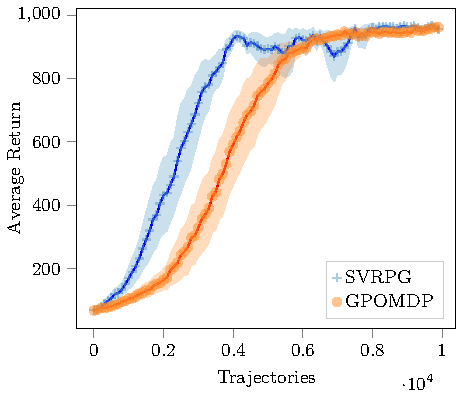
\includegraphics[width=0.75\textwidth]{Images/Experiments/cart_pole_SVRPG_vs_GPOMDP_tex.pdf}
		\vspace{-0.1in}
		\caption{On-line performance over sampled trajectories of \acs{SVRPG} vs G(PO)MDP (batch size set to 10) in the Cart-pole task, with 90\% confidence intervals.}
		\label{fig:cartpole}
	\end{minipage}
	\vspace{-0.15in}
\end{figure*}
\begin{figure*}[h]
	\begin{minipage}[h]{1\textwidth}
		\centering
		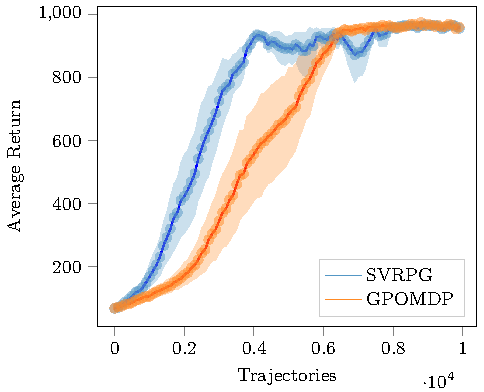
\includegraphics[width=0.75\textwidth]{Images/Experiments/cart_pole_GPOMDP_100_vs_SVRPG.pdf}
		\vspace{-0.1in}
		\caption{On-line performance over sampled trajectories of \acs{SVRPG} vs G(PO)MDP (batch size set to 100) in the Cart-pole task, with 90\% confidence intervals.}
		\label{fig:cartpole100}
	\end{minipage}
	\vspace{-0.15in}
\end{figure*}
\newpage
The Swimmer task is a 3D continuous-control locomotion task over a plane. This task is more difficult than cart-pole. In particular, the longer horizon and the more complex dynamics can have a dangerous impact on the variance of importance weights.

\begin{figure*}[h]
	\begin{minipage}[h]{1\textwidth}
		\centering
		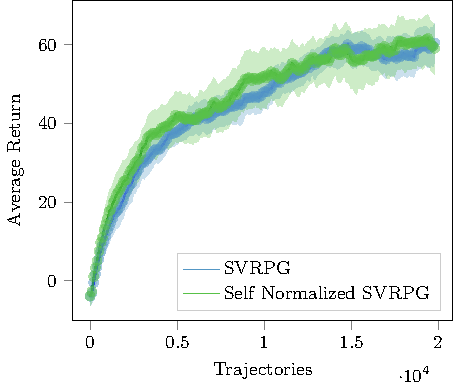
\includegraphics[width=0.75\textwidth]{Images/Experiments/swimmer_self_normalized_SVRPG_vs_SVRPG_tex.pdf}
		\vspace{-0.1in}
		\caption{On-line performance over sampled trajectories of self-Normalized \acs{SVRPG} vs unbiased \acs{SVRPG} in the Swimmer task, with 90\% confidence intervals.}
		\label{fig:swimmertwo}
	\end{minipage}
	\vspace{-0.15in}
\end{figure*}

 In this case, the self-normalization technique proposed in Section \ref{sec:prac} brings an improvement (even if not statistically significant), as shown in Figure \ref{fig:swimmertwo}.
\begin{figure*}[h]
	\begin{minipage}[h]{1\textwidth}
		\centering
		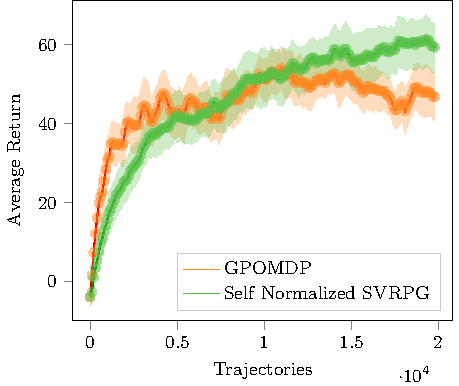
\includegraphics[width=0.75\textwidth]{Images/Experiments/swimmer_self_normalized_SVRPG_vs_GPOMDP_tex.pdf}
		\vspace{-0.1in}
		\caption{On-line performance over sampled trajectories of self-Normalized \acs{SVRPG} vs G(PO)MDP (batch size set to 10) in the Swimmer task, with 90\% confidence intervals}
		\label{fig:swimmerone}
	\end{minipage}
	\vspace{-0.15in}
\end{figure*}
\begin{figure*}[h]
	\begin{minipage}[h]{1\textwidth}
		\centering
		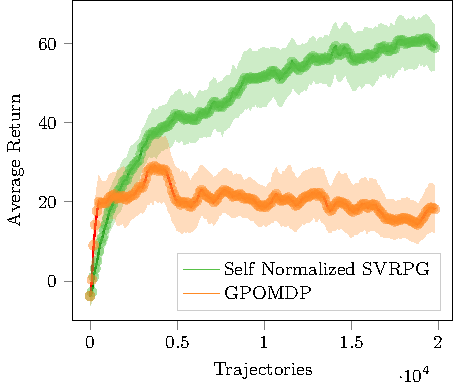
\includegraphics[width=0.75\textwidth]{Images/Experiments/swimmer_GPOMDP_100_vs_SN_SVRPG.pdf}
		\vspace{-0.1in}
		\caption{On-line performance over sampled trajectories of self-Normalized \acs{SVRPG} vs G(PO)MDP (batch size set to 100) in the Swimmer task, with 90\% confidence intervals}
		\label{fig:swimmer100}
	\end{minipage}
	\vspace{-0.15in}
\end{figure*}
% Although the confidence intervals are never disjoint, the average of the self-normalized version is always higher, which we consider enough to employ the variant in the next comparison. 
Figure \ref{fig:swimmerone} shows self-normalized \acs{SVRPG} against G(PO)MDP with batch size set to $10$. Our algorithm outperforms G(PO)MDP for almost the entire learning process. Here, toward the end of the learning process, we note that the improvement becomes statistically significant.

For what concern figure \ref{fig:swimmer100}, where we have self-normalized \acs{SVRPG} versus G(PO)MDP with batch size set to $100$, we can see that our algorithm totally outperforms G(PO)MDP and the difference in performaces is also statistically significant.

Table \ref{tab:1} compares G(PO)MDP and \acs{SVRPG} in terms of the average return computed on the whole learning process, which is a common metric for online learning since it is related to an average regret~\citep[\eg][]{duan2016benchmarking}. This metric can be visualized as the area below the curves. Note that the convergence result in Theorem \ref{theo:convergence} is precisely about the average return. We also report normalized standard deviations and 90\% $t$-confidence intervals.
In both tasks, our algorithm has higher average return and lower normalized standard deviation.
In Cart-pole, disjoint confidence intervals show that the advantage is statistically significant.

\begin{table*}[h]
	\caption{
		\label{tab:1}
		Comparison between G(PO)MDP and \acs{SVRPG} on different tasks. Average return over the whole learning process is reported, together with normalized standard deviation and 90\% confidence intervals.}
	\centering
	\begin{tabular}{@{}lccccccc@{}} 
		\toprule
		\phantom{abc} & \multicolumn{3}{c}{G(PO)MDP $10$} \\
		\cmidrule{2-4}
		\phantom{abc} & Avg Return & Norm. Std & C.I.
		\\\cmidrule{2-4}
		Cart-pole & $618.49$ & $21.09$ & $[579.82, 657.16]$\\
		Swimmer & $45.10$ & $2.37$ & $[40.13, 50.07]$\\
		Half-cheetah & $1263.59$ & $212.73$ & $[810.09, 1717.09]$\\
		\\\cmidrule{2-4}
		\phantom{abc} & \multicolumn{3}{c}{G(PO)MDP $100$} \\
		\cmidrule{2-4}
		\phantom{abc} & Avg Return & Norm. Std & C.I.
		\\\cmidrule{2-4}
		Cart-pole & $608.78$ & $28.66$ & $[556.23, 661.33]$\\
		Swimmer & $20.03$ & $2.56$ & $[15.61, 24.46]$\\
		Half-cheetah & $966.59$ & $173.14$ & $[597.49, 1335.69]$\\
		\\\cmidrule{2-4}
		\phantom{abc} & \multicolumn{3}{c}{SVRPG}
		\\\cmidrule{2-4}
		\phantom{abc} & Avg Return & Norm. Std & C.I.
		\\\cmidrule{2-4}
		Cart-pole & $736.31$ & $16.51$ & $[706.04, 766.57]$\\
		Swimmer & $46.48$ & $2.86$ & $[40.49, 52.46]$\\
		Half-Cheetah & $1397.07$ & $66.74$ & $[1254.78, 1539.36]$\\
		\bottomrule
	\end{tabular}
	\vspace{-0.05in}
\end{table*}

\subsection{Preliminary Results on Actor-Critic.}\label{subsec:actorcritic} %As mentioned, 
Another variance-reduction technique in policy gradient consists in using baselines or \textit{critics}. This tool is orthogonal to the methods described in this composition, and the theoretical results of \hyperref[chap:convergence]{Chapter 4} are general in this sense. In the experiments described so far, we compared against the so-called \textit{actor-only} G(PO)MDP, \ie without the baseline. To move towards a more general understanding of the variance issue in policy gradient, we also test \acs{SVRPG} in an \textit{actor-critic} scenario. To do so, we consider the more challenging MuJoCo~\citep{todorov2012mujoco} Half-cheetah task, a 3D locomotion task that has a larger state-action space than Swimmer. Table \ref{tab:1} also reports the comparison between \acs{SVRPG} and G(PO)MDP\footnote{\citet{duan2016benchmarking} report results on REINFORCE. However, inspection on \textit{rllab} code and documentation reveals that it is actually \ac{PGT} \citep{sutton2000policy}, which is equivalent to G(PO)MDP \citep[shown by][]{peters2008reinforcement}. Using the name REINFORCE in a general way is inaccurate, but widespread.} on Half-cheetah using the critic suggested in \cite{duan2016benchmarking} for both algorithms. More precisely, this critic is a linear state-value function estimator. 
The (time-varying) feature encoding for the linear baseline is:
\begin{align*}
\vphi(s,t)=[s, s \odot s, 0.01t, (0.01t)^2, (0.01t)^3,1],
\end{align*}
where $s\in\mathbb{R}^d$ is the state vector and $\odot$ is the element-wise product. The baseline is then:
\[
b(s_t,a_t) = \boldsymbol{\lambda}^T\vphi(s_t,t).
\]
The baseline is fitted from scratch at each policy gradient iteration, with least squares, to match state-value function $V^{\pi}(s)$.
When used with \acs{SVRPG}, the critic parameter $\boldsymbol{\lambda}$ is updated only at the snapshot. Table \ref{tab:1} shows promising results, meaning that a combination of the baseline usage and \acs{SVRG}-like variance reduction can yield an improvement that the two techniques alone are not able to achieve. For a more thorough evaluation on Half-Cheetah, together with table \ref{tab:1}, also see figure \ref{fig:hcone} and figure \ref{fig:hctwo}. In the former figure we see how our algorithm has a lot less variance and a higher mean even though the confidence intervals are not disjoint. Whereas in the latter figure we can clearly see how the self-normalization can improve the performance of our algorithm. Furthermore, for completeness, we also show in figure \ref{fig:hc100} G(PO)MPD with batch size set to $100$ against \acs{SVRPG}. Here our algorithm has a better performance accross all the learning process. More over this difference becomes statistically significant after half of the learning process itself. 
\begin{figure*}[h]
	\vspace{1in}
	\begin{minipage}[h]{1\textwidth}
		\centering
		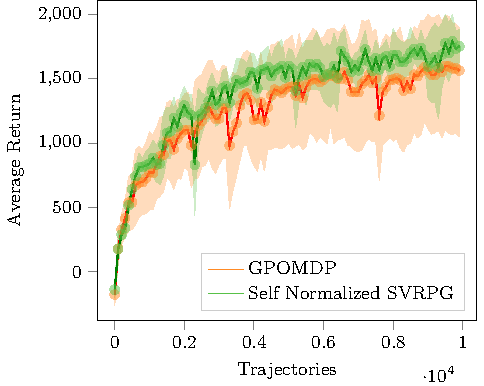
\includegraphics[width=0.75\textwidth]{Images/Experiments/half_cheetah_Self_Normalized_SVRPG_vs_GPOMDP.pdf}
		\vspace{-0.1in}
		\caption{On-line performance over sampled trajectories of self-Normalized \acs{SVRPG} vs G(PO)MDP (batch size set to 10) in the Half-Cheetah task, with 90\% confidence intervals}
		\label{fig:hcone}
	\end{minipage}
	\vspace{-0.15in}
\end{figure*}

\begin{figure*}[h]
	\begin{minipage}[h]{1\textwidth}
		\centering
		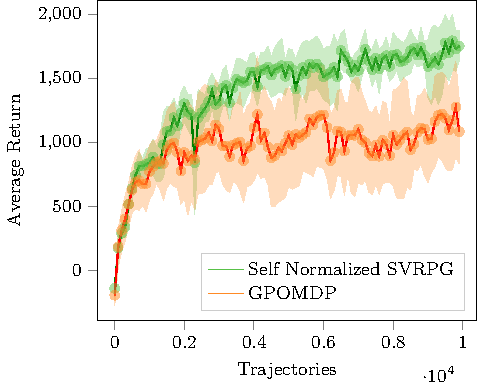
\includegraphics[width=0.75\textwidth]{Images/Experiments/half_cheetah_GPOMDP_100_vs_SN_SVRPG.pdf}
		\vspace{-0.1in}
		\caption{On-line performance over sampled trajectories of self-Normalized \acs{SVRPG} vs G(PO)MDP (batch size set to 100) in the Half-Cheetah task, with 90\% confidence intervals}
		\label{fig:hc100}
	\end{minipage}
	\vspace{-0.15in}
\end{figure*}
\newpage

\begin{figure*}[h]
	\begin{minipage}[h]{1\textwidth}
		\centering
		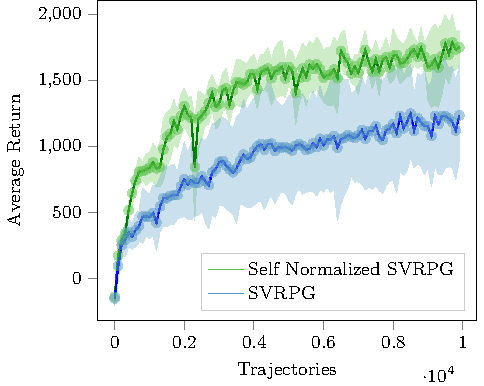
\includegraphics[width=0.75\textwidth]{Images/Experiments/half_cheetah_SVRPG_vs_SN_SVRPG.pdf}
		\vspace{-0.1in}
		\caption{On-line performance over sampled trajectories of self-Normalized \acs{SVRPG} vs unbiased \acs{SVRPG} in the Half-Cheetah task, with 90\% confidence intervals.}
		\label{fig:hctwo}
	\end{minipage}
	\vspace{-0.15in}
\end{figure*}

\subsection{Exploratory Results on Other Gradient Estimators}\label{subsec:oge}
Another preliminary attempt was made using different gradient estimators in our algorithm. Therefore equation \eqref{E:svrpg.estimate.batch} has been rearranged in order to get new gradient estimators. Here we report the obtained expressions:

\begin{align}\label{E:svrpg.b.version}
	\blacktriangledown J(\vtheta_{t}) &:= v_t= \wh{\nabla}_N J(\wt{\vtheta})\\ \notag
	& \quad{} + 
		\frac{1}{B} \sum_{i=0}^{B-1} \left[
		\omega(\tau_i|\wt{\vtheta}, \vtheta_t)g(\tau_i|\wt{\vtheta}) - g(\tau_i|\wt{\vtheta})
		\right]
\end{align}
where the sampling distribution is $\pi_{\wt{\vtheta}}$ for the mini-batch terms.
\begin{align}\label{E:svrpg.c.version}
	\blacktriangledown J(\vtheta_{t}) &:= v_t= \frac{1}{N}\sum_{i=1}^{N} \omega(\tau_i|\wt{\vtheta}, \vtheta_t)g(\tau_i|\wt{\vtheta})\\\notag & \quad{} + 
		\frac{1}{B} \sum_{i=0}^{B-1} \left[
		g(\tau_i|\vtheta_t) - g(\tau_i|\wt{\vtheta})
		\right]
\end{align}
where the sampling distribution is $\pi_{\vtheta_t}$ for the mini-batch terms.\newline
Since equation \ref{E:svrpg.b.version} has $\pi_{\wt{\vtheta}}$ as sampling distribution in the sub-iterations, we can avoid sampling from the environment randomly picking $B$ trajectories from those ones obtained for the snapshot, hence saving a lot of data. Note that in this way we have introduced a bias which, however, is legitimated by the huge data saving. Furthermore, being this version off policy, we have the importance weights exactly on the term we want an estimate of. This latter feature could be dangerous in tasks with a lot of stochasticity, because the variance on the importance weights could dramatically ruin the quantity we want to estimate. Whereas equation \ref{E:svrpg.c.version} has the importance weights binded to the term with $N$ trajectories, which better shrinks the variance contribution of the weights themselves \wrt when they were binded to the term with $B$ trajectories. Notice that the two terms that cancel in expected value do not mean anything when considered alone. From now on we refer to our algorithm based on equation \ref{E:svrpg.b.version} as \acs{SVRPG} B version if it does not reuse the trajectories of the snapshot and \acs{SVRPG} BR if it does, whereas we refer to our algorithm based on equation \ref{E:svrpg.c.version} as \acs{SVRPG} C version.\newline
The results coming from the usage of these new estimators within our algorithm are not satisfying except for the equation \ref{E:svrpg.b.version} version in cart-pole (see \hyperref[chap:appendix]{Appendix A} for the experimental results). These outcomes are due to the fact that the work performed in these directions is currently at an early stage and would need a more thoughtful approach in order to have a chance to make them properly work in practice.

\vspace{-0.05in}